\documentclass[xcolor=dvipsnames]{beamer}
%\documentclass[handout,xcolor=dvipsnames,pdftex,hyperref={colorlinks=false}]{beamer}

% == Packages for beamer
\usepackage{xcolor}
\usepackage{graphicx}
\usepackage{fancybox}
\usepackage{hyperref}
\usepackage{amsmath,amssymb,amsfonts,bm}
\usepackage{wasysym}
\usepackage{colortbl}
\usepackage[english]{babel}
\usepackage{times}
\usepackage[T1]{fontenc}
\usepackage{multirow}

% == Other Packages
\usepackage{rotating}
\usepackage{latexsym}
\usepackage{ulem}
\usepackage{subfigure}
\newenvironment{Shaded}{}{}


% == theme & colors
\usetheme{Warsaw}  % Jens' previous
\usepackage{helvet}
\definecolor{someblue}{rgb}{0,.1,0.8}

% == New Commands
% = For general typesetting
\newcommand\spacingset[1]{\renewcommand{\baselinestretch}{#1}\small\normalsize}
\renewcommand\r{\right}
\renewcommand\l{\left}

\newcommand\makegaps{\addtolength{\itemsep}{.25\baselineskip}}
\newcommand\makebiggaps{\addtolength{\itemsep}{.5\baselineskip}}
\newcommand\smallunskip{\vspace{-.25\baselineskip}}
\newcommand\medunskip{\vspace{-.5\baselineskip}}
\newcommand\bigunskip{\vspace{-\baselineskip}}

\newcommand{\VerbBar}{|}
\newcommand{\VERB}{\Verb[commandchars=\\\{\}]}
% Add ',fontsize=\small' for more characters per line
\newcommand{\KeywordTok}[1]{\textcolor[rgb]{0.00,0.44,0.13}{\textbf{{#1}}}}
\newcommand{\DataTypeTok}[1]{\textcolor[rgb]{0.56,0.13,0.00}{{#1}}}
\newcommand{\DecValTok}[1]{\textcolor[rgb]{0.25,0.63,0.44}{{#1}}}
\newcommand{\BaseNTok}[1]{\textcolor[rgb]{0.25,0.63,0.44}{{#1}}}
\newcommand{\FloatTok}[1]{\textcolor[rgb]{0.25,0.63,0.44}{{#1}}}
\newcommand{\CharTok}[1]{\textcolor[rgb]{0.25,0.44,0.63}{{#1}}}
\newcommand{\StringTok}[1]{\textcolor[rgb]{0.25,0.44,0.63}{{#1}}}
\newcommand{\CommentTok}[1]{\textcolor[rgb]{0.38,0.63,0.69}{\textit{{#1}}}}
\newcommand{\OtherTok}[1]{\textcolor[rgb]{0.00,0.44,0.13}{{#1}}}
\newcommand{\AlertTok}[1]{\textcolor[rgb]{1.00,0.00,0.00}{\textbf{{#1}}}}
\newcommand{\FunctionTok}[1]{\textcolor[rgb]{0.02,0.16,0.49}{{#1}}}
\newcommand{\RegionMarkerTok}[1]{{#1}}
\newcommand{\ErrorTok}[1]{\textcolor[rgb]{1.00,0.00,0.00}{\textbf{{#1}}}}
\newcommand{\NormalTok}[1]{{#1}}


% = For stats & econometrics
\renewcommand{\epsilon}{\varepsilon}
\newcommand\ud{\mathrm{d}}
\newcommand\dist{\buildrel\rm d\over\sim}
\newcommand\ind{\stackrel{\rm indep.}{\sim}}
\newcommand\iid{\stackrel{\rm i.i.d.}{\sim}}
\newcommand\logit{{\rm logit}}
\newcommand\cA{\mathcal{A}}
\newcommand\cN{\mathcal{N}}
\newcommand\E{\mathbb{E}}
\newcommand\V{\mathbb{V}}
\newcommand\cJ{\mathcal{J}}
\newcommand\y{{\bm y}}
\newcommand\Y{{\bm Y}}
\newcommand\X{{\bm X}}
\newcommand\x{{\bm x}}
\newcommand\eps{{\bm\varepsilon}}
\newcommand\zero{{\bm 0}}
\newcommand\be{{\bm\beta}}
\renewcommand\b{{\bm b}}
\newcommand\C{{\bm C}}
\newcommand\D{{\bm D}}
\newcommand\I{{\bm I}}
\newcommand\Z{{\bm Z}}
\newcommand\eeta{{\bm \eta}}
\newcommand{\Var}{\mathrm{Var}}
\newcommand{\Cov}{\mathrm{Cov}}

\DeclareMathOperator*{\argmin}{argmin}

\DeclareMathOperator*\plim{plim}
\DeclareMathOperator\rank{rank}
\newcommand\indep{\protect\mathpalette{\protect\independenT}{\perp}}
\DeclareMathOperator{\sgn}{sgn}
\def\independenT#1#2{\mathrel{\rlap{$#1#2$}\mkern2mu{#1#2}}}

%\documentclass[xcolor=dvipsnames]{beamer}
%%\usecolortheme[named=OliveGreen]{structure}
%\usecolortheme[named=Blue]{structure}
%%\usetheme{Rochester}
%\setbeamertemplate{items}[ball]
%\setbeamertemplate{blocks}[rounded][shadow=true]
%\usepackage{xcolor}
%\usepackage{colortbl}
%\setbeamertemplate{navigation symbols}{}
%\usepackage{amssymb}
%\usepackage{amsmath}
%\usepackage[english]{babel}
%% or whatever
%
%%\usepackage[latin1]{inputenc}
%% or whatever
%
%%\mode<presentation>
%%{
%\usetheme{Warsaw}
%  % or ...
%  %\usecolorheme{albatross}
%%  \setbeamercovered{transparent}
%  % or whatever (possibly just delete it)
%%}

%\usepackage{helvet}
%%\usepackage[T1]{fontenc}
%% Or whatever. Note that the encoding and the font should match. If T1
%% does not look nice, try deleting the line with the fontenc.

\newtheorem{assumption}{Assumption}
\newtheorem{iass}{Identification Assumption}
\newtheorem{ires}{Identfication Result}
\newtheorem{estm}{Estimand}
\newtheorem{esti}{Estimator}

%\newcommand{\indep}{{\bot\negthickspace\negthickspace\bot}}
\newcommand{\notindep}{{\bot\negthickspace\negthickspace\bot}{\negthinspace
  \negmedspace \negthickspace \negthickspace \diagup
  \;}}

\newcommand{\bs}{\boldsymbol}
\newcommand{\mb}{\mathbf}
\newcommand{\real}{\mathbb{R}}
\renewcommand{\u}{\ensuremath{\mb{u}}}
\renewcommand{\v}{\ensuremath{\mb{v}}}
\newcommand{\U}{\ensuremath{\mb{U}}}
\newcommand{\M}{\ensuremath{\mb{M}}}
\renewcommand{\b}{\ensuremath{\bs{\beta}}}
\newcommand{\e}{\ensuremath{\bs{\epsilon}}}
\newcommand{\bhat}{\ensuremath{\hat{\bs{\beta}}}}
\newcommand{\XX}{\ensuremath{\X'\X}}
\newcommand{\XXinv}{\ensuremath{\left(\XX\right)^{-1}}}
\newcommand{\hatsig}{\ensuremath{\hat{\sigma}^2}}
\newcommand{\sig}{\ensuremath{\sigma^2}}
\newcommand{\hatmat}{\ensuremath{\X \XXinv \X'}}
\newcommand{\ehat}{\ensuremath{\hat{\e}}}
\newcommand{\tr}{\text{tr}}
\newcommand{\Sig}{\ensuremath{\bs{\Sigma}}}
\newcommand{\SigInv}{\ensuremath{\bs{\Sigma^{-1}}}}
\newcommand{\W}{\ensuremath{\mb{W}}}

%\usepackage{fixltx2e} % provides \textsubscript
%\ifxetex
%%  \usepackage{fontspec,xltxtra,xunicode}
%  \usepackage{mathspec,xltxtra,xunicode}
%  \defaultfontfeatures{Mapping=tex-text,Scale=MatchLowercase}
%  \setmainfont[Ligatures={Common,TeX}]{Gill Sans}
% % \setmathfont[Digits, Latin]{Gill Sans}
% \setmathfont{LucidaBrightMathOT.otf}
%
%\else
%  \ifluatex
%    \usepackage{fontspec}
%    \defaultfontfeatures{Mapping=tex-text,Scale=MatchLowercase}
%  \else
%    \usepackage[utf8]{inputenc}
%  \fi
%\fi

\AtBeginSection[]
{
  \begin{frame}<beamer>
    \frametitle{Outline}
    \tableofcontents[currentsection]
  \end{frame}
}
%\AtBeginSubsection[]
%{
%  \begin{frame}<beamer>
%    \frametitle{Outline}
%    \tableofcontents[currentsection,currentsubsection]
%  \end{frame}
%}

\title[]{Selection on Observables III: Propensity Scores, Weighting, Regression}
\subtitle[ ]{PS200C, Spring 2025}
\author[Hazlett]{Chad Hazlett }
\institute[UCLA]{UCLA\\[1ex]
  \texttt{chazlett@ucla.edu}
}
\date{}

\definecolor{dgreen}{rgb}{0,.6,0.8}
\useoutertheme{infolines}

\begin{document}

\subject{Talks}
\AtBeginSection[]
{
  \begin{frame}<beamer>
    \frametitle{Outline}
    \tableofcontents[currentsection]
  \end{frame}
}

%\AtBeginSubsection[]
%{
%  \begin{frame}<beamer>
%    \frametitle{Outline}
%    \tableofcontents[currentsection,currentsubsection]
%  \end{frame}
%}

\begin{frame}
  \titlepage
\end{frame}


%\begin{frame}{Project check-in}
%
%\begin{enumerate}
%\item What is sensitivity analysis?
%
%\item What kind of papers should you be looking for? Where?
%
%\item Replication: 
%\begin{itemize}
%\item original vs. OLS 
%\item yes, use whatever replication data and code you can!
%\end{itemize}
%\item Order of operations, replication vs. sensitivity focus
%\end{enumerate}
%\end{frame}

\begin{frame}{Roadmap}
\begin{enumerate}
\item Theory: Potential outcomes, identification, key quantities
\item Randomization
\begin{itemize}
\item difference in means, variance estimation
\item covariate adjustment
\item blocking
\end{itemize}
\item Selection on Observables
\begin{itemize}
\item sub-classification
\item matching (on $X$)
\item weighting (on $X$)
\item matching and weighting on $Pr(D=1)$ (propensity scores)
\item regression 
\end{itemize}
\item Instrumental Variables
\item Regression Discontinuity
\item Difference in Differences and Synthetic Control
\item Sensitivity and Bounds
\end{enumerate}
\end{frame}

\begin{frame}{We have to keep saying this...}

\begin{block}{Assumption: Conditional Ignorability}
$$ \{ Y_i(0), Y_i(1)\} \ \indep \ D_i \mid X_i = x \quad \text{for any} \quad x \in \mathcal{X} $$
\smallskip
\footnotesize
(a.k.a. exogeneity, unconfoundedness, selection on observables, no omitted variables) \\
\end{block}
\bigskip
\small
\onslide<2-> So we have ``experiments'' within each stratum of $X$, but how to estimate an average effect as if we did it strata-wise then averaged? (``conditioning on $X$'')\\
\small
\begin{itemize}
\item<3-> We took very literal approach with sub-classification and matching
\item<4-> Now, let's think about re-weighting in ways that make the overall distribution of treated and control more similar
\item<5-> This will allow us to estimate things as if we have done so conditionally on $X$ then averaged over some density in $X$
\end{itemize}
\end{frame}

%
%
%\begin{frame}{Back to Propensity Scores}
%\small
%\onslide<1-> We just saw a kind of weight that has only to do with getting balance on $X$ w/o contemplating a treatment assignment model. \\
%\bigskip
%\onslide<2-> But recall an option we saw earlier: Nature gave us
%\footnotesize
%\[\int \E[Y_i|D_i=1,X_i]\textcolor{Orange}{p(X_i|D=1)} dx- \int \E[Y_i|D_i=0,X_i]\textcolor{Green}{p(X_i|D_i=0)} dx \]
%\small
%\medskip
%\onslide<4-> Weighting by \textcolor{Blue}{$\frac{p(D_i)}{p(D_i|X_i)}$}  or equivalently $\frac{p(X_i)}{p(X_i|D_i)}$ gives
%\footnotesize
%\onslide<5->
%\scriptsize
%\begin{align*}
%\int \E[Y_i|D_i=1,X_i]\frac{\textcolor{Orange}{p(X|D=1)}\textcolor{Blue}{p(D_i=1)}}{\textcolor{Blue}{p(D_i=1|X_i)}} dx  &- \int \E[Y_i|D_i=0,X_i]\frac{\textcolor{Green}{p(X|D_i=0)}\textcolor{Blue}{p(D_i=0)}}{\textcolor{Blue}{p(D_i=0|X_i)}} dx \\
%= \int \E[Y_i|D_i=1,X_i]\textcolor{Red}{p(X_i)}dx &- \int \E[Y_i|D_i=0,X_i]\textcolor{Red}{p(X_i)}dx
%\end{align*}
%\footnotesize
%\onslide<6-> We call $p(D_i=1|X_i)$ the propensity score, and $\frac{p(D_i)}{p(D_i|X_i)}$ the (stabilized) inverse propensity score weights (\textcolor{Red}{IPW}).
%\end{frame}

\begin{frame}{Propensity Scores: The conventional motivation}
\small 
\begin{itemize}
\item May be tough to get close matches on $X_i$ when multi-dimensional
\item What if you could just match on a one-dimensional summary? 
\end{itemize}
\begin{block}{Conditioning on the Propensity Score}
Under SOO and common support,
\vspace{-.1in}
\[ \{ Y_i(0), Y_i(1)\} \ \indep \ D_i \mid \pi(X_i)\]
\end{block}

\onslide<2-> The intuition: 
\begin{itemize}
\item Among those with $\pi(X_i)=c$, you have$Pr(D_i=1)=c$ no matter what differences in $X_i$ you see.
\item That is,  $D_i$ does not depend upon $X_i$, conditionally on $\pi(X_i)$.
\item Once $D_i$ no longer depends on $X_i$, it also no longer depends on $\{Y_{1i},Y_{0i}\}$ (SOO).
\item So its like random experiments within each stratum of $\pi(X_i)$.
\end{itemize}
\end{frame}
 
% one thinks of the propensity score, $\pi_i = p(D_i=1|X_i)$, as a way of simplifying the matching problem:
%\footnotesize
%\begin{itemize}
%\item it is hard to get close matches on $X_i$ if $X_i$ is multi-dimensional
%\item  but what if you could just match on a one-dimensional summary of some kind? 
%\item The propensity score: 
%\end{itemize}
%\begin{block}{Conditioning on the Propensity Score}
%Under SOO and common support,
%\vspace{-.1in}
%\[ \{ Y_i(0), Y_i(1)\} \ \indep \ D_i \mid \pi(X_i)\]
%\end{block}
%\onslide<3-> Why?
%\small
%\begin{itemize}
%\item Imagine a cell with constant $Pr(D=1)$: all units have same $Pr(D=1)$ regardless of $Y_{1i}$, or $Y_{0i}$. 
%\item See next for more rigor.
%\end{itemize}
%\end{frame}

\begin{frame}{Identification with Propensity Scores}
\begin{Proof}
\small
Show that $\Pr(D = 1|Y_0, Y_1, \pi(X)) = \Pr(D = 1|\pi(X)) = \pi(X)$, implying
independence of $(Y_0,Y_1)$ and $D$ conditional on $\pi(X)$.
\begin{eqnarray*}
\Pr(D=1|Y_1,Y_0,\pi(X))&=&\E[D|Y_1,Y_0,\pi(X)]\\ \pause
&=&\E\left[\E[D|Y_1,Y_0,X]|Y_1,Y_0,\pi(X)\right] \mbox{ (LIE) }\\ \pause
&=&\E\left[\E[D|X]|Y_1,Y_0,\pi(X)\right] \mbox{ (SOO) } \\\pause
&=&\E\left[\pi(X)|Y_1,Y_0,\pi(X)\right] \\ \pause
&=&\pi(X)
\end{eqnarray*}
Using a similar argument
\begin{eqnarray*}
\Pr(D=1|\pi(X))&=&\E[D|\pi(X)]=\E[\E[D|X]|\pi(x)]\\ \pause
&=&\E[\pi(X)|\pi(X)]=\pi(X)
\end{eqnarray*}
therefore $\Pr(D=1|Y_1,Y_0,\pi(X))=\Pr(D=1|\pi(X))$
\end{Proof}
\end{frame}

\begin{frame}{Using Propensity Scores}
\onslide<1->  First, estimate $P(D_i=1|X_i) = \hat{\pi_i}$, e.g. by logit.  Then condition on it:
\small
\begin{itemize}
\item<2-> Matching:
\footnotesize 
\begin{itemize}
\item may need a \textit{caliper} to trim cases without common support
\item or, trim cases with extreme pscores by hand
\item but beware, this changes your estimand
\end{itemize}  
\small
\item<3-> Weighting
\footnotesize
\begin{itemize}
\item<4-> Simple IPW weights:  $\frac{1}{p(D_i|X_i)}=\frac{1}{D_i \pi_i + (1-D_i)(1-\pi_i)}$
\item<5-> Stabilized IPW weights: $\frac{p(D_i)}{p(D_i|X_i)}$ 
\item<6-> But if using weights, check how extreme they get and how few units are doing most of the work
\end{itemize}
\end{itemize}
\end{frame}

\begin{frame}{Using Propensity Scores}
\onslide<1-> \textcolor{Blue}{Pros:}
\footnotesize
\begin{itemize}
\item Just one thing to match on
\item Ignores imbalance on $X$'s that do not predict $D$...very helpful for large $P$
\item Will give you balance (``balancing property''), but \textit{only in expectation} and if correctly estimated
\end{itemize}
\medskip
\normalsize
\onslide<2-> \textcolor{Blue}{Cons:}
\footnotesize
\begin{itemize}
\item If balancing property seen as the \textit{goal} of pscores -- by that metric it often under-performs. (See King \& Nielsen 2015)
\item Requires correct model and estimation of the propensity score!
\item Extreme weights can cause large bias (so check)
\end{itemize}
\medskip
\normalsize
\onslide<3-> IPW weights that also guarantee balance? 
\footnotesize 
\begin{itemize}
\item \textcolor{Blue}{Covariate balancing propensity scores} (CBPS; Imai, Ratkovic 2014)\\
\item For continuous treatments, \textcolor{Blue}{CBGPS} (Fong, Hazlett, Imai 2017)
\end{itemize}
\end{frame}

%\begin{frame}
%Now to \texttt{R}...
%\vspace{-.2in}
%\begin{figure}[ht] \centering
%    
\includegraphics[scale=.55]{all_blattman.pdf}
%\end{figure}
%\end{frame}


\begin{frame}[fragile]
\frametitle{Using Propensity Scores: Blattman \& Annan}
\scriptsize
\begin{verbatim}
pi.out = glm(abd~age+fthr_ed+mthr_ed+hh_size96+orphan96+C_ach+C_akw+
			C_ata+C_kma+C_oro+C_pad+C_paj+C_pal,data=dat,family="binomial"(link=logit))

matchout.pi=Match(Y=dat$educ,Tr=dat$abd,X=pi.out$fit,estimand="ATT")
summary(matchout.pi)

#Check balance
mb.out.pi =MatchBalance(match.out=matchout.pi,abd~age+fthr_ed+
			mthr_ed+hh_size96+orphan96+C_ach+C_akw+C_ata+C_kma+
			C_oro+C_pad+C_paj+C_pal,data=dat)

btest_after_pi=baltest.collect(mb.out.pi,var.names=varnames,after=TRUE)

balancecompare.pi=cbind(btest[,c("mean.Tr","mean.Co","T pval",
"KS pval")],btest_after_pi[,c("mean.Tr","mean.Co","T pval","KS pval")])
\end{verbatim}
\end{frame}

\begin{frame}[fragile]
\frametitle{Using Propensity Scores: Blattman \& Annan}
\scriptsize
\begin{verbatim}
 balancecompare.pi
          mean.Tr mean.Co T pval KS pval mean.Tr mean.Co T pval KS pval
age         21.37   20.15   0.00    0.00   21.37   21.04   0.27    0.17
fthr_ed      5.76    6.07   0.27    0.87    5.76    5.60   0.48    0.09
mthr_ed      2.09    2.49   0.09    0.35    2.09    2.40   0.11    0.20
hh_size96    8.09    8.70   0.06    0.04    8.09    8.02   0.79    0.03
orphan96     0.08    0.08   0.90      NA    0.08    0.11   0.07      NA
C_ach        0.15    0.11   0.13      NA    0.15    0.17   0.60      NA
C_akw        0.16    0.08   0.00      NA    0.16    0.17   0.62      NA
C_ata        0.10    0.20   0.00      NA    0.10    0.09   0.55      NA
C_kma        0.15    0.12   0.19      NA    0.15    0.16   0.87      NA
C_oro        0.05    0.14   0.00      NA    0.05    0.05   0.95      NA
C_pad        0.12    0.12   0.98      NA    0.12    0.09   0.10      NA
C_paj        0.15    0.10   0.06      NA    0.15    0.15   0.91      NA
C_pal        0.11    0.13   0.51      NA    0.11    0.13   0.45      NA
\end{verbatim}
\end{frame}

\begin{frame}[fragile]
\frametitle{Using Propensity Scores: Blattman \& Annan}
\onslide<1-> Weighting on the propensity scores (stabilized IPW):
\scriptsize
\begin{verbatim}
ps=pi.out$fit
D=dat$abd
PrD=mean(D)
IPW= (D*PrD+(1-D)*(1-PrD))/(D*ps+(1-D)*(1-ps))

#Good to check how crazy the weights are:
plot(density(IPW))
\end{verbatim}
\vspace{-.25in}
\begin{center}

\includegraphics[width=.65\textwidth]{IPWdensity.pdf}%
\end{center}
\end{frame}

\begin{frame}[fragile]
\frametitle{How does $p(\pi_i)$ look before/after weighting?}
\vspace{-.3in}
\onslide<2-> 
\scriptsize
\begin{verbatim}
plot(density(pi.out$fit[D==1], weight=IPW[D==1]/sum(IPW[D==1])))
lines(density(pi.out$fit[D==0], weight=IPW[D==0]/sum(IPW[D==0])),lwd=2)
legend("topleft", legend=c("treated","controls"), lty=c(1,2))
\end{verbatim}
\vspace{-.25in}
\begin{center}

\includegraphics[width=.5\textwidth]{pscores_pre.pdf}%

\includegraphics[width=.5\textwidth]{pscores_post.pdf}%
\end{center}
\end{frame}

\begin{frame}[fragile]
\frametitle{Check Omnibus Balance}
\onslide<2-> 
\tiny
\begin{verbatim}
omnibus.bal = lm(abd~age+fthr_ed+mthr_ed+hh_size96+orphan96+
                   C_ach+C_akw+C_ata+C_kma+C_oro+C_pad+C_paj+C_pal, data=dat) 
summary(omnibus.bal) 
#R2=0.08, F-statistic: 5.585 on 12 and 728 DF,  p-value: 3.303e-09
\end{verbatim}
\onslide<3->
\begin{verbatim}
omnibus.bal.ipw = lm(abd~age+fthr_ed+mthr_ed+hh_size96+orphan96+
                   C_ach+C_akw+C_ata+C_kma+C_oro+C_pad+C_paj+C_pal, 
                   weight=IPW, data=dat) 
summary(omnibus.bal.ipw)

Coefficients: (1 not defined because of singularities)
              Estimate Std. Error t value Pr(>|t|)    
(Intercept)  6.138e-01  1.058e-01   5.804 9.69e-09 ***
age          5.474e-04  3.691e-03   0.148    0.882    
fthr_ed     -4.053e-04  5.352e-03  -0.076    0.940    
mthr_ed     -2.116e-04  6.628e-03  -0.032    0.975    
hh_size96    4.875e-04  4.689e-03   0.104    0.917    
orphan96     3.979e-03  6.873e-02   0.058    0.954    
---
Multiple R-squared:  0.0002747,	Adjusted R-squared:  -0.0162 
F-statistic: 0.01667 on 12 and 728 DF,  p-value: 1
\end{verbatim}
\onslide<4-> 
\normalsize
\begin{center}
Yay!
\end{center}
\end{frame}

\begin{frame}[fragile]
\frametitle{Estimating the ATE with IPW weights}
\scriptsize
\begin{verbatim}
lm.out.naive = lm(educ~abd, data=dat) 
lm.out.ipw = lm(educ~abd, weight=IPW, data=dat) 
lm.out.ipw2=lm(educ~abd+age+fthr_ed+mthr_ed+hh_size96+orphan96+
    C_ach+C_akw+C_ata+C_kma+C_oro+C_pad+C_paj+C_pal,weight=IPW,data=dat) 
\end{verbatim}

% Table created by stargazer v.5.1 by Marek Hlavac, Harvard University. E-mail: hlavac at fas.harvard.edu
% Date and time: Sun, May 03, 2015 - 07:15:58 PM
\vspace{-.1in}
\begin{table}[!htbp] \centering 
  %\caption{} 
  \label{} 
\begin{tabular}{@{\extracolsep{5pt}}lccc} 
\\[-1.8ex]\hline 
\hline \\[-1.8ex] 
 & \multicolumn{3}{c}{\textit{Dependent variable:}} \\ 
\cline{2-4} 
\\[-1.8ex] & \multicolumn{3}{c}{educ} \\ 
\\[-1.8ex] & (1) & (2) & (3)\\ 
\hline \\[-1.8ex] 
 abd & $-$0.595$^{***}$ & $-$0.726$^{***}$ & $-$0.735$^{***}$ \\ 
  & (0.218) & (0.220) & (0.210) \\ 
  & & & \\ 
 Constant & 7.416$^{***}$ & 7.499$^{***}$ & 6.113$^{***}$ \\ 
  & (0.172) & (0.174) & (0.610) \\ 
  & & & \\ 
\hline \\[-1.8ex] 
Observations & 741 & 741 & 741 \\ 
R$^{2}$ & 0.010 & 0.014 & 0.128 \\ 
Adjusted R$^{2}$ & 0.009 & 0.013 & 0.112 \\ 
Residual Std. Error (df = 739) & 2.876 & 2.904 & 2.754 \\ 
%F Statistic  & 7.457$^{***}$ & 10.862$^{***}$ & 8.192$^{***}$ \\ 
\hline 
\hline \\[-1.8ex] 
\textit{Note:}  & \multicolumn{3}{r}{$^{*}$p$<$0.1; $^{**}$p$<$0.05; $^{***}$p$<$0.01} \\ 
\end{tabular} 
\end{table} 
\end{frame}


\begin{frame}{Balance Plot after IPW}
\begin{center}
%%
\includegraphics[width=.5\textwidth]{pscores_pre.pdf}%

\includegraphics[width=.8\textwidth]{all_blattman.pdf}
\end{center}
\end{frame}


\begin{frame}{A different view on weighting}
\onslide<1-> For my money I prefer to think of weights as follows:\\
\begin{itemize}
\item<2-> We have conditional treatment effects in each stratum of $X$:
\small
\[\E[\tau|X] = \textcolor{Blue}{\E[Y_i|D_i=1,X_i]-\E[Y_i|D_i=0,X_i]  } \]
\smallskip
\normalsize
\item<4-> We wish we could take this $\E[\tau|X]$ and average it up over some distribution, say \textcolor{Red}{$p(X)$}:
\small
\begin{align*}
\E_X\E[\tau|X] &= \int \textcolor{Blue}{\E[Y_i|D_i=1,X_i]-\E[Y_i|D_i=0,X_i]}\textcolor{Red}{p(X)} dx \\
&= \int \textcolor{Blue}{\E[Y_i|D_i=1,X_i]}\textcolor{Red}{p(X)} dx- \textcolor{Blue}{\int \E[Y_i|D_i=0,X_i]}\textcolor{Red}{p(X)} dx \\
&= \text{\footnotesize mean for treated minus controls when same \textcolor{Red}{density, p(X)} }
\end{align*}
\end{itemize}
\small
\begin{center}
\onslide<5-> Preview: we could get this if we could ``move'' the treated/control to both have $\textcolor{Red}{p(X)}$ instead of $p(X|D=1)$ and $p(X|D=0)$
\end{center}
\end{frame}

\begin{frame}{What does it mean for weights to ``move a distribution''?}
\onslide<1-> 
%\begin{column}{.48\textwidth}
            \begin{center}
            \begin{figure}
            \vspace{-.2in}
            
\includegraphics[scale=.25]{density_treated_control.pdf}
             
\includegraphics[scale=.25]{density_treated_wcontrol.pdf}
            \end{figure}
            \end{center} 
 %           \end{column}
%\begin{column}{.48\textwidth}        
%\begin{center}
%
%\begin{figure}   
%\vspace{-.2in}
%			 
\includegraphics[scale=.28]{density_treated_wcontrol.pdf}\\
%            \end{figure}
%            			 \end{center}
% %           \end{column}
%% \end{columns}
\footnotesize
\onslide<2-> Here we move a control distribution to look like treated (as you would for ATT), but the point is about the role of weights in shifting a distribution.\\
\end{frame}

\begin{frame}{What weights achieve this?}
\small
\onslide<1-> For ATE, we \textcolor{Red}{wish we could} average over $p(X)$ for treated and controls,
\footnotesize
\[ \int \textcolor{Blue}{\E[Y_i|D_i=1,X_i]}\textcolor{Red}{p(X)} dx- \textcolor{Blue}{\int \E[Y_i|D_i=0,X_i]}\textcolor{Red}{p(X)} dx \] \\
\small
\onslide<2-> But nature gives us this DIM:
\footnotesize
\[\int \E[Y_i|D_i=1,X_i]\textcolor{Orange}{p(X_i|D=1)} dx- \int \E[Y_i|D_i=0,X_i]\textcolor{Green}{p(X_i|D_i=0)} dx \]
\small
\medskip
\onslide<3-> Consider weighting by \textcolor{Blue}{$\frac{p(X_i)}{p(X_i|D_i)}$}: (aka $\frac{p(D_i)}{p(D_i|X_i)}$)
\footnotesize
\onslide<4->
\begin{align*}
\E[\hat{\tau}_{IPW}] &= \int \E[Y_i|D_i=1,X_i]\frac{\textcolor{Orange}{p(X|D=1)}\textcolor{Blue}{p(X_i)}}{\textcolor{Blue}{p(X_i|D_i=1)}} dx \\
&   \quad \quad -\int \E[Y_i|D_i=0,X_i]\frac{\textcolor{Green}{p(X|D_i=0)}\textcolor{Blue}{p(X_i)}}{\textcolor{Blue}{p(X_i|D_i=0)}} dx \\
&= \int \E[Y_i|D_i=1,X_i]\textcolor{Red}{p(X_i)}dx- \int \E[Y_i|D_i=0,X_i]\textcolor{Red}{p(X_i)}dx \\
\end{align*} \\
\end{frame}


\begin{frame}{The duality of weights}
\small
\onslide<1-> Those weights ($\frac{p(D_i)}{p(D_i|X_i)}$) are exactly the (stabilized) IPW weights! \\
\bigskip
\onslide<2-> That is, the weights that get you balance are also the weights you'd get with the (real) IPW. \\
\bigskip
\onslide<3-> This gives us two (flawed) ways forward
\footnotesize
\begin{itemize}
\item try to compute the IPWs...but this requires a model, $\widehat{p(D_i|X_i)}$
\medskip
\item try to get balance on $X$...but you have to pick some specific functions of $X$ to balance
\medskip
\item In other words: choosing weights by IPW and by balancing are the same in theory but will be different in practice with different weaknesses.
\end{itemize}
\normalsize 
\small
\bigskip
\onslide<4-> The first has a longer history and we've talked about it, let's get to the second...\\
\end{frame}



\begin{frame}{Weighting for balance}

\onslide<1-> In these approaches, forget about trying to model the treatment, just choose weights that give you ``balance'':\\

\small
\begin{itemize}
\item<3-> Ideally you want to get $p(X|D=1)$ to equal $p(X|D=0)$. 
\smallskip
\item<4-> Often people settle for equal means alone, i.e. $\E[X|D=0] \approx \E[X|D=1]$.
\smallskip
\item<5-> Though we can try to get equal means on $X^2$, $X_1 X_2$, etc. as well
\smallskip
\item<6-> It turns out that these get you unbiased ATT estimates when $Y_{0i}$ is linear in the things you get mean balance on
\end{itemize}
\end{frame}

\begin{frame}{Weighting for covariate balance}
\small
\onslide<1-> To be explicit: find weights on control units s.t. the mean of $X$ (or other functions of $X$) among controls matches that of treated. \\
\bigskip
\onslide<2-> Resulting weights can be used to get weighted difference in means, or applied to any outcome model (e.g. regression)
\small
\begin{itemize}
\item<3-> Could also move treated to controls (\textcolor{Blue}{for what estimand?}), or move both to overall means (\textcolor{Blue}{for what estimand?})
\item<4-> You can often find perfect mean balance, no iteration
%\item<5-> Main downside: only getting balance on means or other included functions
\item<5-> Standard errors are still an open question. Bootstrap likely okay.
\end{itemize}
\bigskip
\footnotesize
\onslide<6-> Get equal means: entropy balancing (Hainmueller, 2011), \texttt{ebal}\\
\medskip
\onslide<7-> To get multivariate (smoothed) balance, $\hat{p}(X|D=0)=\hat{p}(X|D=1)$, Kernel Balancing (\texttt{kbal}, see my website).
\end{frame}

\begin{frame}{Balance on Blattman data with Ebal}
\vspace{-.35in}
\begin{figure}[ht] \centering
    
\includegraphics[scale=.8]{ebal_blattman.pdf}
\end{figure}

\end{frame}


%%%%%%%%%%%%%%%%%%%%%%%%%%%%%%%%%%%%%%%%%%%%%%%%%%%%%%%%%
\subsection*{Regression}

\begin{frame}{Model-based Estimation of Causal Effects}
\small
\onslide<1-> Regression popular to ``control for'' variables. Does this allow causal inference? \\
\medskip
\onslide<2-> Take the quantity: \\
\[\E[\tau(x)] = \E[Y_{1i} \mid X_i=x] - \E[Y_{0i} \mid X_i=x] \]
\onslide<3-> Which under CI is identifiable with estimator:
\[ \E[\tau(x)] = \E[Y_i\mid D_i=1, X_i=x] - \E[Y_i\mid D_i=0, X_i=x] \] \\

%\onslide<4-> And we can use it to compute things like: 
%$$ \tau_{ATE} \ = \ \E[\hat\tau(x)] \quad \text{and} \quad \tau_{ATT} \ = \ \E[\hat\tau(x)\mid D_i=1] $$

\onslide<5-> A \alert{model-based} approach for estimating causal effects:
\footnotesize
\begin{itemize}
\item<6-> Suppose $\E[Y_{0i}|X_i]=\E[Y_i \mid D_i=0, X_i]=\beta_0+\gamma^{\top}X_i$
\item<7-> ...and $\E[Y_{1i}|X_i]=\E[Y_i \mid D_i=1, X_i]=\beta_0+\beta_1+\gamma^{\top}X_i$
\item<8-> Which means $\beta_1= \E[\tau(X)]$ 
\item<9-> As single model: 
$$ \E[Y_i\mid D_i, X_i] \ = \ \beta_0 + \beta_1D_i + \gamma^\top X_i, $$
\end{itemize}
%\onslide<4-> Does this work?
\end{frame}

\begin{frame}{OLS as an Estimator of Causal Effects}
\small
\onslide<1-> When is $\hat{\beta}_{OLS}$ a good estimator of $\tau_{ATE}$?\\
\medskip
\onslide<2-> We might posit two assumptions:
\begin{enumerate}
\item[(1)]<3-> \alert{Constant treatment effect}. We assumed
\begin{itemize}
\item $\E[\tau(X)]$ is always one number... 
\item i.e., constant (expected) treatment effects (by strata of $X$)
\end{itemize}
\item[(2)]<4-> \alert{Linearity}: %We assert that
%\[ \E[Y_{id} | X_i, D_i]=\beta_0 + \beta_1 D_i  + \gamma^{\top}X_i   \quad \text{for} \quad d = 0, 1 \]
By which we really mean
 \begin{align*}
 	Y_{id} &= \beta_0 + \beta_1 D_i  + \gamma^{\top}X_i + \epsilon_i \quad \text{with } \E[\epsilon_i|X_i, D_i]=0
 \end{align*}
\end{enumerate}
\vspace{-.2in}
\onslide<5-> Where $\E[\epsilon_i|X_i, D_i]=0$ (the ``conditional independence assumption'')\\
\onslide<6-> Noting that (2) implies (1) there are 3 possible scenarios:
\footnotesize
\begin{enumerate}
\addtolength{\itemsep}{-.25\baselineskip}
\item Both (1) and (2) are true.
\item Only (1) is true.
\item Neither (1) nor (2) is true.
\end{enumerate}
\end{frame}

\begin{frame}{Case 1: Constant Effect w/ Linear Potential Outcomes}
\onslide<1->
\textbf{Result}: 
If treatment effect is constant across units and potential outcomes are linear in $X_i$, then the OLS estimate of $\beta_1$ in the following regression model
$$ Y_i \ = \ \beta_0 + \beta_1 D_i + \gamma^\top X_i + \epsilon_i $$
is an unbiased and consistent estimator of $\tau_{ATE}$.

\bigskip
\onslide<2-> \textbf{Proof} (just how we got here):
\footnotesize
\begin{align*}
\E[\beta_1] &= \E_x \E[Y_i|D_i=1, X_i]-\E[Y_i|D_i=0, X_i] \quad \text{(correct specification)}\\
&= \E_x \E[Y_{1i}|X_i]- \E[Y_{0i}|X_i] \quad \text{(SOO)}\\
&= \E_x \tau(X) \\
&= \tau \quad \text{(constant effect assumption)}
\end{align*}
\medskip
\onslide<3-> Note equivalence:  CI+linearity $\rightarrow$ $\epsilon$ cannot be related to $D$ given $X$ (CIA):
%\bigskip
%\onslide<3-> Note that CI implies the conditional independence between $D_i$ and $\epsilon_i$:
$$ \l\{Y_i(1), Y_i(0)\r\} \ \indep \ D_i \mid X_i \quad \Longrightarrow \quad \epsilon_i \ \indep \ D_i \mid X_i $$
%
%Because this implies the zero conditional mean assumption, $\hat\beta_{OLS}$ is an unbiased and consistent estimator of $\beta_1$, which is equal to $\tau_{ATE}$ (and $\tau_i$). \qed
%
\end{frame}


\begin{frame}{Case 2: Constant Effect w/ Unknown Functional Form}
\small
\onslide<1-> Linearity is a very strong assumption in most practical situations.\\
\medskip
\onslide<2-> What if $\E[Y_i(d)|X_i, D_i]$ is an unknown, nonlinear function of $X$ and $D$ but we use OLS? \\
\medskip
\onslide<3-> Recall that OLS is still the \alert{best linear predictor} in terms of MSE:
$$\hat\beta_{OLS} \ = \ \argmin_{\hat\beta_1} \ \E\l[(\alert{Y_i} - \hat\beta_0 - \hat\beta_1 D_i - \hat\gamma^\top X_i)^2\r] $$
\medskip
\onslide<4-> Implies $\hat\beta_{OLS}$ is \alert{best linear approximation} to the population regression function:
$$\hat\beta_{OLS} \ = \ \argmin_{\hat\beta_1} \ \E\l[\l(\alert{\E[Y_i\mid D_i,X_i]} - \hat\beta_0 - \hat\beta_1 D_i - \hat\gamma^\top X_i\r)^2\r] $$
\footnotesize
\vspace{-.2in}
\begin{itemize}
\item<5-> $\therefore$ we say ``$\hat\beta_{OLS}$ is best linear approximation to the true treatment effect'', whatever the true functional form is.
\item<6-> This approximation may or may not be good! Danger of mis-specification bias.
\item<7-> More flexible models (nonlinear, semi-/non-parametric, etc.) are a good idea
\end{itemize}
\end{frame}

\begin{frame}{Case 3: Heterogeneous Treatment Effects}
\small
\onslide<1-> We typically cannot assume constant treatment effects. Is this a problem?\\
\medskip
\onslide<2-> Recall the subclassification estimator for the \alert{ATE}:
\footnotesize
\[ \hat\tau_{ATE} \ = \ \sum_{x \in \mathcal{X}} \l\{ \E[Y_i\mid D_i=1, X_i=x] - \E[Y_i\mid D_i=0, X_i=x] \r\} \alert{\Pr(X_i=x)} \]
\small
\onslide<3-> Similarly, the subclassification estimator for the \alert{ATT}:
\footnotesize

\[\hat\tau_{ATT} \ = \ \sum_{x \in \mathcal{X}} \l\{ \E[Y_i\mid D_i=1, X_i=x] - \E[Y_i\mid D_i=0, X_i=x] \r\} \alert{\Pr(X_i=x\mid D_i=1)} \]
\medskip

\onslide<4-> \textbf{Result:} The OLS estimator can be written as a subclassification estimator, where the weights come from \alert{conditional variances of $D_i$} in each subgroup: 
\onslide<5->
\scriptsize
\[ \hat\beta_{OLS} \ = \ \sum_{x \in \mathcal{X}} \l\{ \E[Y_i\mid D_i=1, X_i=x] - \E[Y_i\mid D_i=0, X_i=x] \r\} \frac{\textcolor{Blue}{\Var(\hat{D}_i\mid X_i=x)}\textcolor{Red}{\Pr(X_i=x)}}{\textcolor{Blue}{\sum_{x'}\Var(\hat{D}_i\mid X_i=x')\Pr(X_i=x')}} \]
\smallskip
\begin{itemize}
\item \textcolor{Blue}{Intuition:} OLS ``learns more'' from strata of $X$ where $\pi_X$ closer to 0.50.
\item think about what this means for your estimate, especially with lack of overlap
\item This is from Angrist and Pischke. It depends on $D$ being linear in $X$. For more general weights, see my Shinkre \& Hazlett.
\end{itemize}
\end{frame}

\begin{frame}{OLS as a Subclassification Estimator}
\small
\begin{center}
{\renewcommand{\arraystretch}{1.25}
\begin{tabular}{lcc} \hline
Estimator & Weights for Subgroups & Unbiased for \\ \hline
$\hat\tau_{ATE}$ & $\Pr(X_i=x)$ & $\tau_{ATE}$ \\
$\hat\tau_{ATT}$ & $\Pr(X_i=x\mid D_i=1)$ & $\tau_{ATT}$ \\
$\hat\beta_{OLS}$ & {\scriptsize $\displaystyle\frac{\Var(\hat{D}_i\mid X_i=x)\Pr(X_i=x)}{\sum_{x'}\Var(\hat{D}_i\mid X_i=x')\Pr(X_i=x')}$} & ``$\tau_\text{CVW-ATE}$'' \\ \hline
\end{tabular}
}
\end{center}
\footnotesize
\begin{itemize}
\item<1-> With heterogeneous treatment effects, OLS provides an unbiased estimator for a {\it conditional-variance-weighted average treatment effect}.
\smallskip
\item<2-> Estimand has a causal meaning, but difficult to interpret. Not the ATE or ATT.
\smallskip
\item<3-> Note: $\Var(\hat{D}_i\mid X_i=x) = \hat{\pi}(x)(1-\hat{\pi}(x))$. Thus,
\begin{itemize}
\item<3-> what happens when $\hat{\pi}_i$ is 0 or 1?
\item<4-> largest weights for strata $\hat{\pi}_i$ close to $0.5$,
\end{itemize}
\item<5-> This result assumes discrete $X$s, but intuition holds for continuous $X$s.
\end{itemize}
\end{frame}

\begin{frame}{Improvements over pooled OLS}
\small
\begin{itemize}
\item<1-> \textbf{Imputation}: use regression to impute missing potential outcomes. E.g.  Estimate $\E[Y_{0i}|X_i]$ and use as counterfactuals for observed $Y_{1i}$. Can weight each pairwise difference as you like. Aka g-computation, T-learner.
\item<2-> \textbf{Interactive} (i.e. Lin). Include interaction of $X$ with $D$ to allow separate slope for $\E[Y(0)|X]$ and $\E[Y(1)|X]$.
\end{itemize}
\bigskip
\onslide<3-> It turns out these are precisely the same thing!\\
\begin{itemize}
\item Both relax your (modeling) assumption from ``Y is linear in D and X'' (which implies constant treatment effects) to ``Y(1) is linear in X, and Y(0) is linear in X'', which we call ``separate linearity'' (Shinkre \& Hazlett)
\item Unless you somehow care about $\tau_{CVW-ATE}$ as such, the only reason to use OLS without interaction/imputation is that it would be more efficient in the case where you really do have constant treatment effects. 
\end{itemize}
\end{frame}

\begin{frame}
\frametitle{Combining Regression, Matching and Weighting}
\onslide<1-> The different logics of matching, weighting, and regression can be combined to improve finite-sample performance or robustness: \\

\begin{itemize}
\small
\makegaps
\item<2-> Bias-corrected matching (Abadie and Imbens 2005): 
\footnotesize
	\begin{itemize}
	\makegaps
	\item estimate bias due to unequal $Y_{0i}$ of matched units due to imperfect match on  $X$'s. 
	\item subtract it off from the matching estimate for correction
	\end{itemize}
\small
\item<3-> ``Doubly-robust'' estimation by weighted regression:
\footnotesize
	\begin{itemize}
	\makegaps
	%\item Use a weighted average of regression and IPW estimators (Robins and Rotnitzky 2001):
	\item Use weighting (e.g. IPW or balancing weights) in a regression that also includes covariates
	\end{itemize}
	\item<4-> Construct estimators that employ both an outcome model and a weighting of residuals from it.
	\begin{itemize}
	\item See especially double-ml (DML), augmented IPW (AIPW), targeted maximum likelihood (tMLE)
	\end{itemize}
	\small
%\item<4-> Matching as nonparametric preprocessing (Ho et al. 2007):
%\footnotesize
%	\begin{itemize}
%	\makegaps
%	\item model-based estimation of causal effect is most likely to go wrong when it involves \alert{extrapolation} due to poor overlap in covariates
%	\item use matching to make treatment and control groups similar
%	\item then run regression models to estimate causal effects
%	\end{itemize}
\end{itemize}
\end{frame}


%\begin{frame}
%\frametitle{Extrapolation and Model Dependence}
%\begin{center}
%\includegraphics[width=.5\textwidth]{images/pic1a}%
%\includegraphics[width=.5\textwidth]{images/pic1b}
%\end{center}
%\end{frame}

\begin{frame}
\frametitle{Summary: Estimation under Conditional Ignorability}
\small
\begin{itemize}
\item<1-> Matching, weighting and regression are used estimate average causal effects when one can assume conditional ignorability
\item<2-> These are estimation strategies; the validity of the identification strategy (SOO) remains a first-order concern
\item<3-> No single method is dominant at the moment, and the tides will change...
\item<4-> My two cents: Ideally the estimator doesn't matter so much; best if you can use 5 different ones and get similar results. Differences in results often point to poor overlap/ model dependency problems that are worth exploring anyway.
%\begin{itemize}
%\item<6-> is there risk of extrapolation due to non-overlap? 
%\item<7-> is there risk you are not doing the conditioning you mean to do? 
%\item<8-> given your actual data -- e.g. whether you have to condition on continuous or categorical variables -- what approach will make most sense to complete the conditioning your ID strategy requires?
%\end{itemize}
%\item Going beyond simple ATE/ATT often requires some modeling, where preprocessing with matching could greatly improve reliability
\end{itemize}

\end{frame}







%other ways to think about weighting:
%the balance we were trying to get...
% getting p(X|D)=p(X) gets you X \indep D. 
%...also known as p(D|X)=p(D)...both imply no longer need 
% to condition on X, you've done it. now

%\subsection{Example: Blattman and Annan (2009)}
%\begin{frame}{Example: Blattman and Annan (2009)}
%\small
%\begin{quote}
%\texttt{The Consequences of
%Child Soldiering. \textit{The Review of Economics and Statistics}.}
%\end{quote}
%\small
%\bigskip
%\onslide<3-> \textcolor{Blue}{Question}: what is the impact of abduction by the rebel group \textit{Lord's Resistance Army} on education? \\
%\bigskip
%\onslide<4-> \textcolor{Blue}{ID Strategy:} SOO. According to the logic by which abduction occurred, \emph{we will assume that abduction is indiscriminate, conditional on age and location.}
%
%\footnotesize
%\begin{quote}
%Abduction was large-scale and seemingly indiscriminate; 60,000 to 80,000 youth are estimated to have been abducted and more than a quarter of males currently aged 14 to 30 in our study region were abducted for at least two weeks...
%
%Youth were typically taken by roving groups of 10 to 20 rebels during night raids on rural homes. Adolescent males appear to have been the most pliable, reliable and effective forced recruits, and so were disproportionately targeted by the LRA. Youth under age 11 and over 24 tended to be avoided and had a high probability of immediate release. 
%\end{quote}
%\end{frame}
%
%\begin{frame}{Example: Blattman and Annan (2009)}
%\small
%\onslide<1-> \textcolor{Blue}{Data}: panel survey of male youth in war-afflicted regions of Uganda. \\
%\footnotesize
%\begin{itemize}
%\item \texttt{abd}: abducted by the LRA (the treatment)
%\item \texttt{c\_ach -- c\_pal:} Location indicators
%\item \texttt{age}: age in years
%\item \texttt{fthr\_ed},\texttt{mthr\_ed} : father's/mother's education (years)
%\item \texttt{orphan96}: indicator if parent's died before 1997
%\item \texttt{hh\_fthr\_frm}: indicator if father is a farmer
%\item \texttt{hh\_size96}: household size in 1996
%\item \texttt{educ}: years of education
%\item \texttt{distress}: index of emotional distress (0-15)
%\item \texttt{logwage}: log of average daily wage earned in last 4 weeks
%\end{itemize}
%\small
%\bigskip
%\onslide<3-> \alert{NB:} \texttt{educ}, \texttt{distress}, and \texttt{logwage} are measured after abduction.\\
%\bigskip
%\onslide<4-> Now, to \texttt{R}.
%\end{frame}


%\subsection{Propensity Scores}\label{propensity-scores}
%
%%\begin{frame}{Review: Law of Iterated Expectations}
%%
%%\begin{definition}
%%A very important property of conditional expectations is:
%%$$
%%\E[Y]=\E[\E[Y|X]]
%%$$
%%since $\E[Y|X]$ is a function of $X$, the outer expectation
%%is taken with respect to the distribution of $X$.
%%\end{definition}
%%
%%Example: \pause 
%%
%%Imagine $Y$=Support and $X$=gender $(1,0)$. Then, the law of iterated
%%expectations tells us: \[
%%\E[Y]=\pause \E[Y|X=1]\cdot \Pr(X=1) + \E[Y|X=0]\cdot \Pr(X=0).
%%\] This means: \medskip
%%\small
%%
%%\begin{tabular}{lcll}
%%Average Support &=& Average Support for men&$\times$ Proportion of men\\
%%               &+& Average Support for women&$\times$ Proportion of women.
%%\end{tabular}
%%
%%\end{frame}
%
%\begin{frame}{Identification with Propensity Scores}
%
%\begin{definition}
%Propensity score is defined as the selection probability conditional on the confounding variables:
%$\pi(X)=\Pr(D=1|X)$
%\end{definition}
%
%\begin{iass}
%\begin{enumerate}
%\item $(Y_1,Y_0) \indep D |X$ (selection on observables)
%\item $0<\Pr(D=1|X)<1$ with probability one (common support)
%\end{enumerate}
%\end{iass}
%
%\begin{ires}
%Under selection on observables we have $(Y_1,Y_0) \indep D| \pi(X)$, ie. conditioning
%on the propensity score is enough to have independence between the treatment indicator and potential outcomes. Implies substantial dimension reduction.
%\end{ires}
%
%\end{frame}
%
%\begin{frame}{Identification with Propensity Scores}
%
%\begin{Proof}
%\small
%Show that $\Pr(D = 1|Y_0, Y_1, \pi(X)) = \Pr(D = 1|\pi(X)) = \pi(X)$, implying
%independence of $(Y_0,Y_1)$ and $D$ conditional on $\pi(X)$.
%\begin{eqnarray*}
%\Pr(D=1|Y_1,Y_0,\pi(X))&=&\E[D|Y_1,Y_0,\pi(X)]\\ \pause
%&=&\E\left[\E[D|Y_1,Y_0,X]|Y_1,Y_0,\pi(X)\right] \mbox{ (LIE) }\\ \pause
%&=&\E\left[\E[D|X]|Y_1,Y_0,\pi(X)\right] \mbox{ (SOO) } \\\pause
%&=&\E\left[\pi(X)|Y_1,Y_0,\pi(X)\right] \\ \pause
%&=&\pi(X)
%\end{eqnarray*}
%Using a similar argument
%\begin{eqnarray*}
%\Pr(D=1|\pi(X))&=&\E[D|\pi(X)]=\E[\E[D|X]|\pi(x)]\\ \pause
%&=&\E[\pi(X)|\pi(X)]=\pi(X)
%\end{eqnarray*}
%therefore $\Pr(D=1|Y_1,Y_0,\pi(X))=\Pr(D=1|\pi(X))$
%\end{Proof}
%
%\end{frame}
%
%\begin{frame}{Matching on the Propensity Score}
%
%\begin{corollary} If $(Y_1,Y_0) \indep D|X$, then
%\begin{eqnarray*}
%\E[Y|D=1,\pi(X)=\bar{\pi}]-\E[Y|D=0,\pi(X)=\bar{\pi}]&=&\\
%\E[Y_1-Y_0|\pi(X)=\bar{\pi}]
%\end{eqnarray*}
%\end{corollary}
%
%Suggests a two step procedure to estimate causal effects under selection
%on observables:
%
%\begin{enumerate}
%\def\labelenumi{\arabic{enumi}.}
%\itemsep1pt\parskip0pt\parsep0pt
%\item
%  Estimate the propensity score $\pi(X)=P(D=1|X)$ (eg. using
%  logit/probit regression, machine learning methods, etc) \pause
%\item
%  Match or subclassify on propensity score.
%\end{enumerate}
%
%\end{frame}
%
%\begin{frame}{Estimating the Propensity Score}
%
%\begin{itemize}
%\itemsep1pt\parskip0pt\parsep0pt
%\item
%  Given selection on observables we have $(Y_1,Y_0) \indep D|\pi(X)$
%  which implies the balancing property of the propensity score: \[
%    \Pr(X|D=1,\pi(X))=\Pr(X|D=0,\pi(X))
%    \] \pause
%\item
%  We can use this to check if our estimated propensity score actually
%  produces balance:
%  $P(X|D=1,\widehat{\pi}(X))=P(X|D=0,\widehat{\pi}(X))$ \pause
%\item
%  To properly model the assignment mechanism, we need to include
%  important confounders correlated with treatment and outcome
%\item
%  Need to find the correct functional form, miss-specified propensity
%  scores can lead to bias. Any methods can be used (probit, logit, etc.)
%\item
%  Estimate $\mapsto$ Check Balance $\mapsto$ Re-estimate $\mapsto$ Check
%  Balance
%\end{itemize}
%
%\end{frame}
%
%\begin{frame}[fragile]{Example: Blattman (2010)}
%
%\footnotesize
%
%\begin{Shaded}
%\begin{Highlighting}[]
%\NormalTok{pscore.fmla <-}\StringTok{ }\KeywordTok{as.formula}\NormalTok{(}\KeywordTok{paste}\NormalTok{(}\StringTok{"abd~"}\NormalTok{,}\KeywordTok{paste}\NormalTok{(}\KeywordTok{names}\NormalTok{(covar),}\DataTypeTok{collapse=}\StringTok{"+"}\NormalTok{)))}
%\NormalTok{abd <-}\StringTok{ }\NormalTok{data$abd}
%\NormalTok{pscore_model <-}\StringTok{ }\KeywordTok{glm}\NormalTok{(pscore.fmla, }\DataTypeTok{data =} \NormalTok{data, }
%  \DataTypeTok{family =} \KeywordTok{binomial}\NormalTok{(}\DataTypeTok{link =} \NormalTok{logit))}
%\NormalTok{pscore <-}\StringTok{ }\KeywordTok{predict}\NormalTok{(pscore_model, }\DataTypeTok{type =} \StringTok{"response"}\NormalTok{)}
%\end{Highlighting}
%\end{Shaded}
%
%\centering
%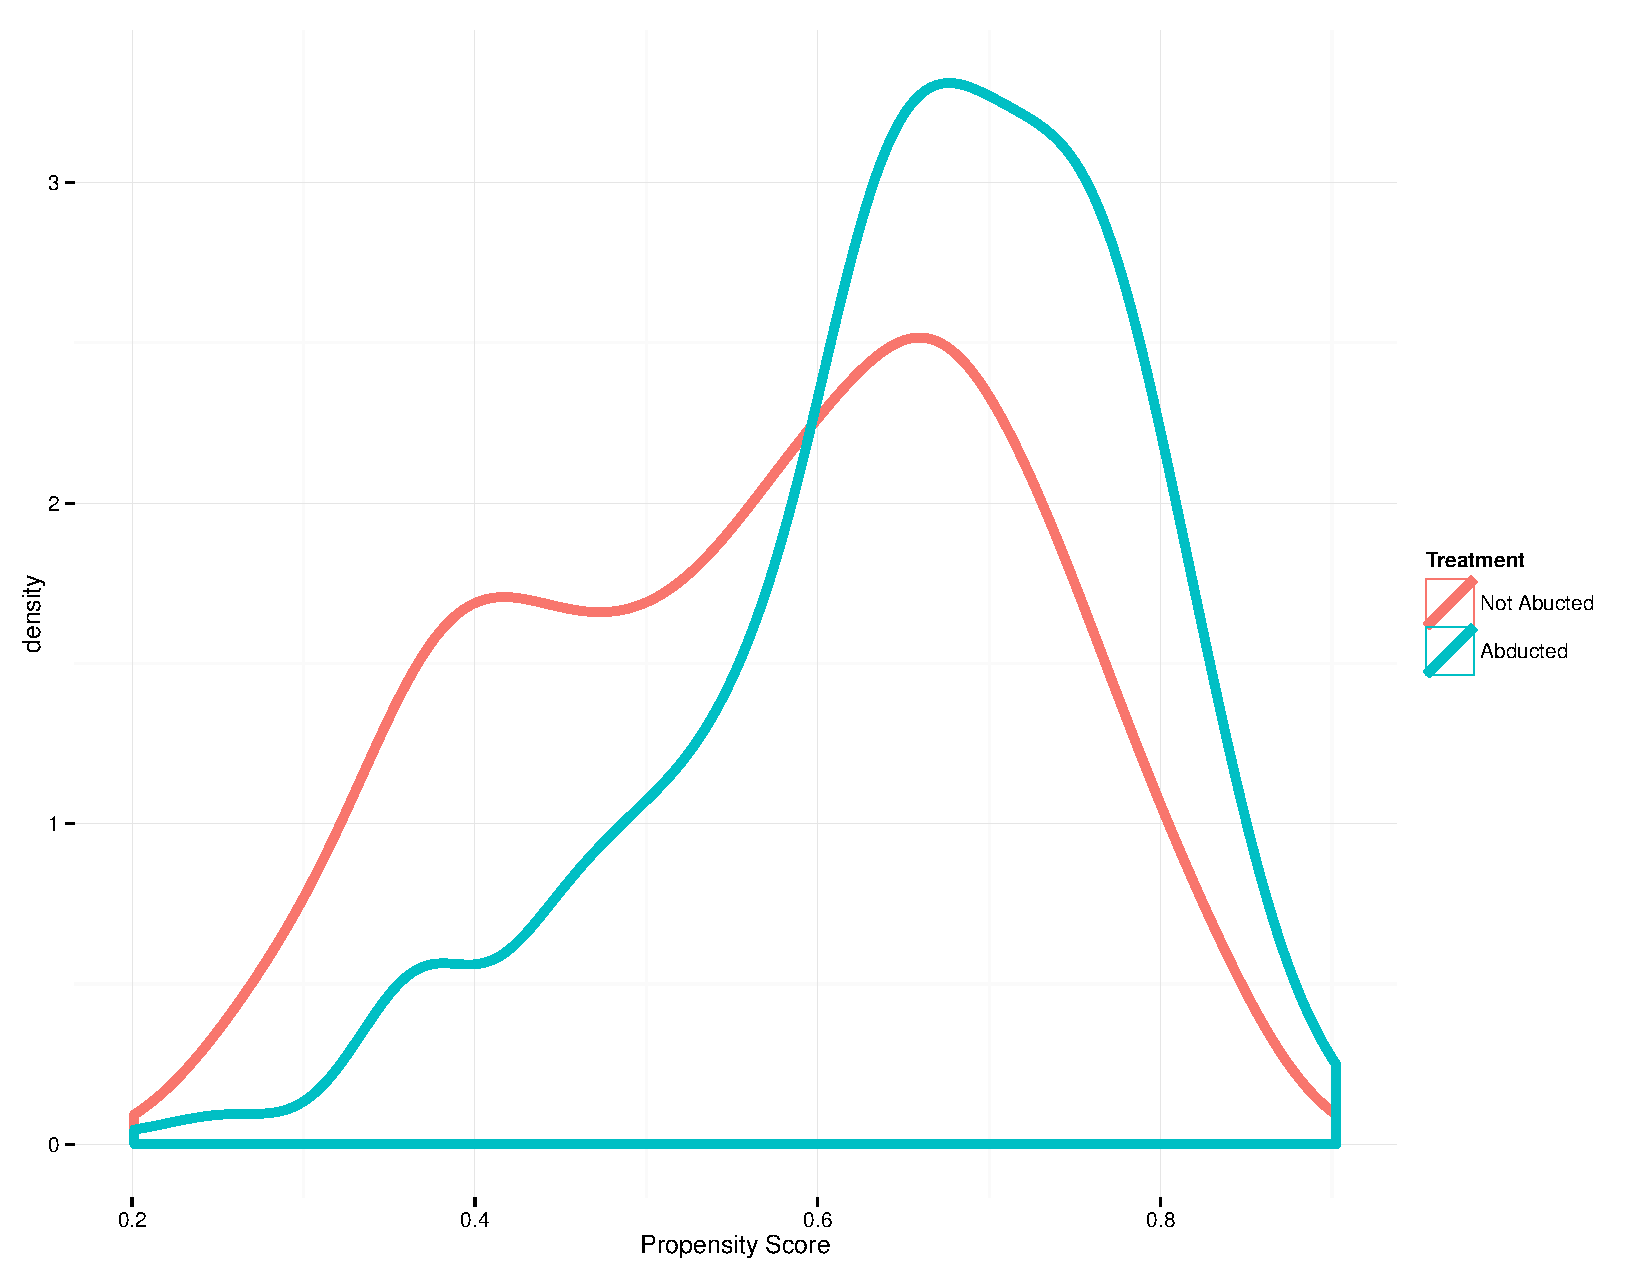
\includegraphics[height = 2.4in]{images/blattman_pscore.pdf}
%
%\end{frame}
%
%\begin{frame}[fragile]{Blattman (2010): Match on the Propensity Score}
%
%\footnotesize
%
%\begin{Shaded}
%\begin{Highlighting}[]
%\NormalTok{match.pscore <-}\StringTok{ }\KeywordTok{Match}\NormalTok{(}\DataTypeTok{Tr=}\NormalTok{abd, }\DataTypeTok{X=}\NormalTok{pscore, }\DataTypeTok{M=}\DecValTok{1}\NormalTok{, }\DataTypeTok{estimand=}\StringTok{"ATT"}\NormalTok{)}
%\end{Highlighting}
%\end{Shaded}
%
%\centering
%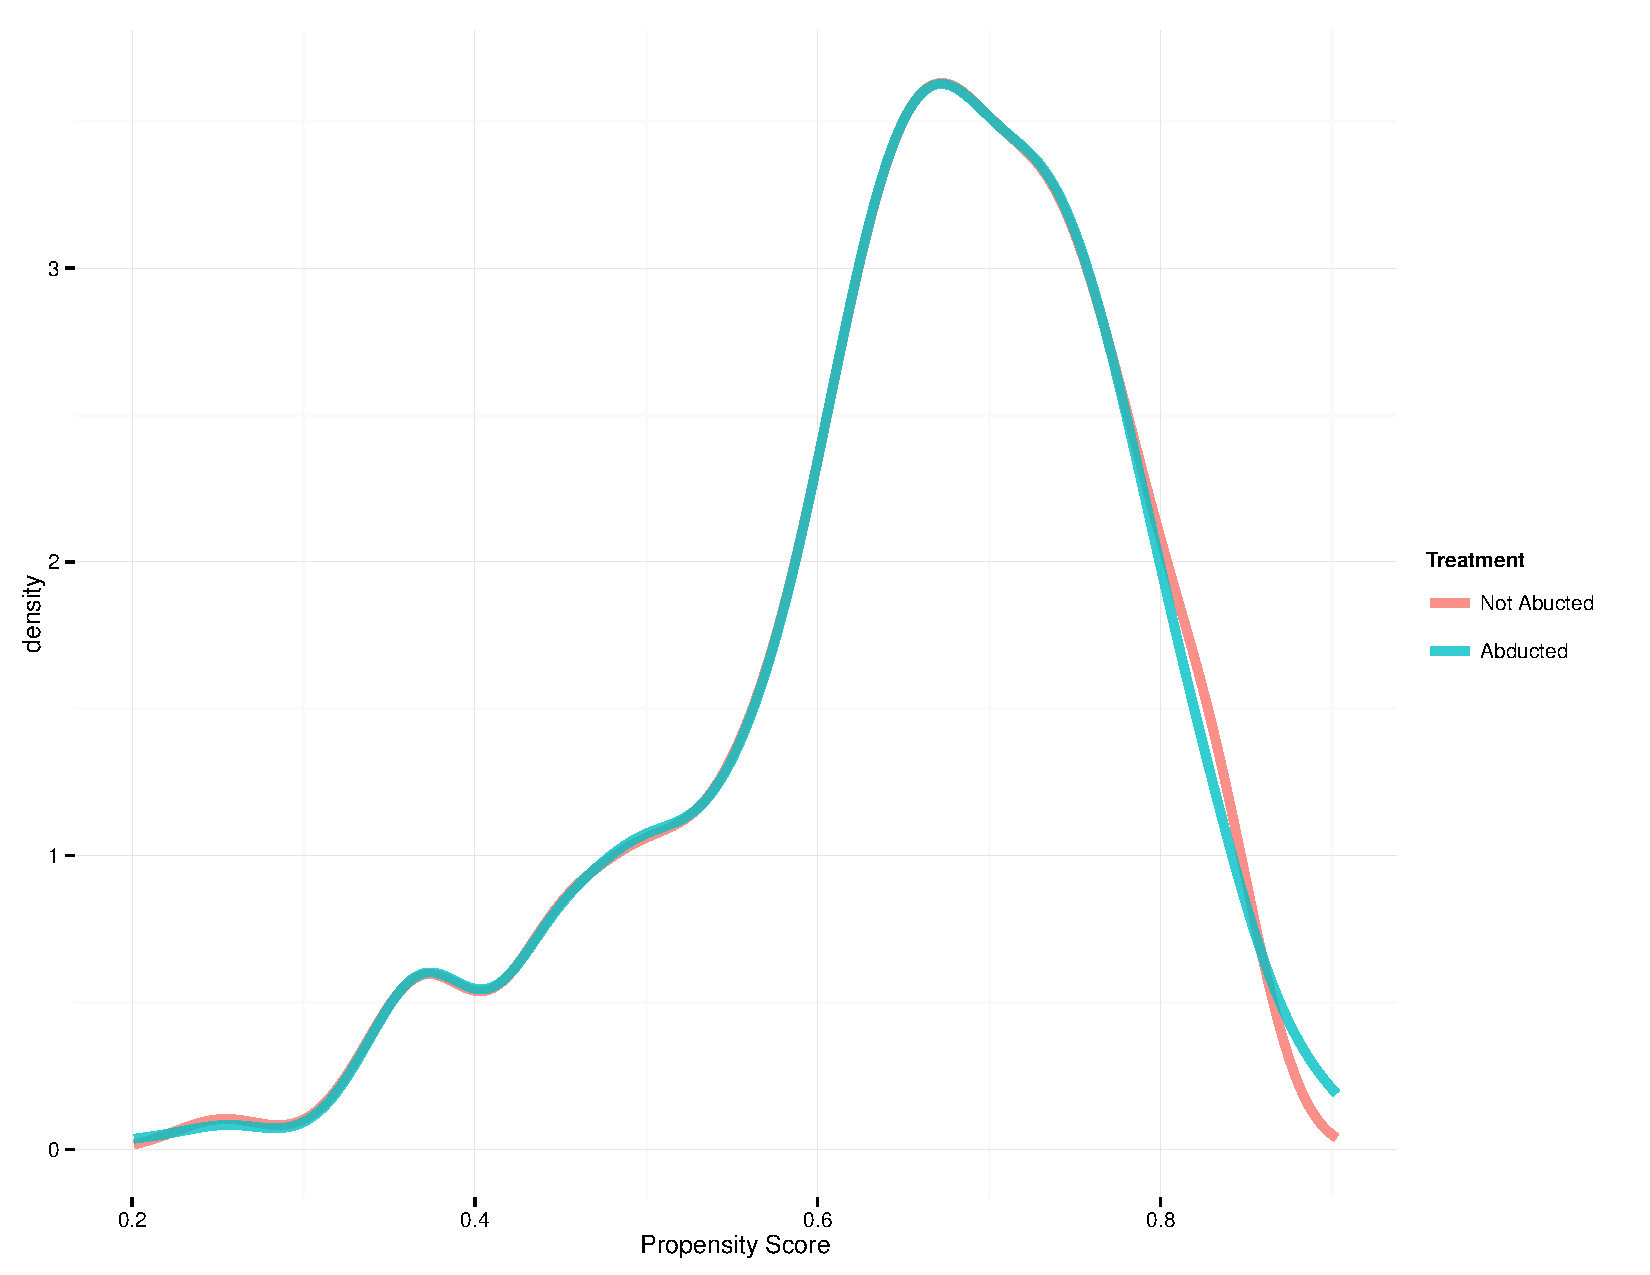
\includegraphics[height = 3in]{images/blattman_pscore_matching.pdf}
%
%\end{frame}
%
%\begin{frame}[fragile]{Blattman (2010): Check Balance}
%
%\footnotesize
%
%\begin{Shaded}
%\begin{Highlighting}[]
%\NormalTok{match.pscore <-}
%\NormalTok{+}\StringTok{ }\KeywordTok{MatchBalance}\NormalTok{(abd ~}\StringTok{ }\NormalTok{age, }\DataTypeTok{data=}\NormalTok{data, }\DataTypeTok{match.out =} \NormalTok{match.pscore)}
%
%\NormalTok{**}\ErrorTok{***}\StringTok{ }\NormalTok{(V1) age **}\ErrorTok{***}
%\StringTok{                       }\NormalTok{Before Matching     After Matching}
%\NormalTok{mean treatment........     }\FloatTok{21.366}          \FloatTok{21.366} 
%\NormalTok{mean control..........     }\FloatTok{20.151}          \FloatTok{20.515} 
%\NormalTok{std mean diff.........     }\FloatTok{24.242}          \FloatTok{16.976} 
%
%\NormalTok{var }\KeywordTok{ratio} \NormalTok{(Tr/Co).....     }\FloatTok{1.0428}         \FloatTok{0.98412} 
%\NormalTok{T-test p-value........  }\FloatTok{0.0012663}       \FloatTok{0.0034409} 
%\NormalTok{KS Bootstrap p-value..      }\FloatTok{0.016}           \FloatTok{0.034} 
%\NormalTok{KS Naive p-value......   }\FloatTok{0.024912}        \FloatTok{0.070191} 
%\NormalTok{KS Statistic..........    }\FloatTok{0.11227}        \FloatTok{0.077899} 
%\end{Highlighting}
%\end{Shaded}
%
%\end{frame}
%
%\begin{frame}[fragile]{Blattman (2010): Mahalanobis Distance Matchng}
%
%\footnotesize
%
%\begin{Shaded}
%\begin{Highlighting}[]
%\NormalTok{match.mah <-}\StringTok{ }\KeywordTok{Match}\NormalTok{(}\DataTypeTok{Tr=}\NormalTok{abd, }\DataTypeTok{X=}\NormalTok{covar, }\DataTypeTok{M=}\DecValTok{1}\NormalTok{, }\DataTypeTok{estimand=}\StringTok{"ATT"}\NormalTok{, }\DataTypeTok{Weight =} \DecValTok{3}\NormalTok{)}
%\KeywordTok{MatchBalance}\NormalTok{(abd ~}\StringTok{ }\NormalTok{age, }\DataTypeTok{data=}\NormalTok{data, }\DataTypeTok{match.out =} \NormalTok{match.mah)}
%
%\NormalTok{**}\ErrorTok{***}\StringTok{ }\NormalTok{(V1) age **}\ErrorTok{***}
%\StringTok{                       }\NormalTok{Before Matching     After Matching}
%\NormalTok{mean treatment........     }\FloatTok{21.366}          \FloatTok{21.366} 
%\NormalTok{mean control..........     }\FloatTok{20.151}          \FloatTok{21.154} 
%\NormalTok{std mean diff.........     }\FloatTok{24.242}          \FloatTok{4.2314} 
%
%\NormalTok{var }\KeywordTok{ratio} \NormalTok{(Tr/Co).....     }\FloatTok{1.0428}          \FloatTok{1.0336} 
%\NormalTok{T-test p-value........  }\FloatTok{0.0012663}      \FloatTok{3.0386e-05} 
%\NormalTok{KS Bootstrap p-value..      }\FloatTok{0.008}           \FloatTok{0.798} 
%\NormalTok{KS Naive p-value......   }\FloatTok{0.024912}         \FloatTok{0.94687} 
%\NormalTok{KS Statistic..........    }\FloatTok{0.11227}        \FloatTok{0.034261} 
%\end{Highlighting}
%\end{Shaded}
%
%\end{frame}
%
%\begin{frame}[fragile]{Blattman (2010): Genetic Matching}
%
%\footnotesize
%
%\begin{Shaded}
%\begin{Highlighting}[]
%\NormalTok{genout <-}\StringTok{ }\KeywordTok{GenMatch}\NormalTok{(}\DataTypeTok{Tr=}\NormalTok{abd,}\DataTypeTok{X=}\NormalTok{covar,}\DataTypeTok{BalanceMatrix=}\NormalTok{covar,}\DataTypeTok{estimand=}\StringTok{"ATT"}\NormalTok{,}
%                  \DataTypeTok{pop.size=}\DecValTok{1000}\NormalTok{)}
%\NormalTok{match.gen <-}\StringTok{ }\KeywordTok{Match}\NormalTok{(}\DataTypeTok{Tr=}\NormalTok{abd, }\DataTypeTok{X=}\NormalTok{covar,}\DataTypeTok{M=}\DecValTok{1}\NormalTok{,}\DataTypeTok{estimand=}\StringTok{"ATT"}\NormalTok{,}\DataTypeTok{Weight.matrix=}\NormalTok{genout)}
%\NormalTok{gen.bal <-}\StringTok{ }\KeywordTok{MatchBalance}\NormalTok{(abd~age,}\DataTypeTok{match.out=}\NormalTok{match.gen,}\DataTypeTok{data=}\NormalTok{covar)}
%
%\NormalTok{**}\ErrorTok{***}\StringTok{ }\NormalTok{(V1) age **}\ErrorTok{***}
%\StringTok{                       }\NormalTok{Before Matching     After Matching}
%\NormalTok{mean treatment........     }\FloatTok{21.366}          \FloatTok{21.366} 
%\NormalTok{mean control..........     }\FloatTok{20.151}          \FloatTok{21.225} 
%\NormalTok{std mean diff.........     }\FloatTok{24.242}          \FloatTok{2.8065} 
%
%\NormalTok{var }\KeywordTok{ratio} \NormalTok{(Tr/Co).....     }\FloatTok{1.0428}          \FloatTok{1.1337} 
%\NormalTok{T-test p-value........  }\FloatTok{0.0012663}         \FloatTok{0.21628} 
%\NormalTok{KS Bootstrap p-value..      }\FloatTok{0.008}           \FloatTok{0.454} 
%\NormalTok{KS Naive p-value......   }\FloatTok{0.024912}         \FloatTok{0.68567} 
%\NormalTok{KS Statistic..........    }\FloatTok{0.11227}        \FloatTok{0.046512} 
%\end{Highlighting}
%\end{Shaded}
%
%\end{frame}
%
%\begin{frame}{Weighting on the Propensity Score}
%
%\small
%Provided that the relevant moments exists, if $Y_1,Y_0\indep D |X$, then
%
%\begin{eqnarray*}
%\tau_{ATE}&=&\E[Y_1-Y_0]=\E\left[
%Y\cdot \frac{D-\pi(X)}{\pi(X)\cdot (1-\pi(X))}
%\right]\\
%\tau_{ATT}&=&\E[Y_1-Y_0|D=1]=\frac{1}{P(D=1)}\cdot \E\left[
%Y\cdot \frac{D-\pi(X)}{1-\pi(X)}
%\right]
%\end{eqnarray*}
%
%\begin{Proof}
%\scriptsize Consider
%\begin{eqnarray*}
%&&\E\left[\left.
%Y \frac{D-\pi(X)}{\pi(X) (1-\pi(X))}\right| X \right]\\
%&=& \E\left[\left.\frac{Y}{\pi(X)} \right|X, D=1 \right] \pi(X) + \E\left[\left.\frac{-Y}{1-\pi(X)}\right|X, D=0\right] (1-\pi(X))\\
%&=& \E[Y|X, D=1] - \E[Y|X, D=0]
%\end{eqnarray*}
%And the results of the proposition follow from integration over $\Pr(X)$ and $\Pr(X|D=1)$.
%\end{Proof}
%
%\end{frame}
%
%\begin{frame}{Weighting on the Propensity Score}
%
%\small
%
%\begin{eqnarray*}
%\tau_{ATE}&=&\E[Y_1-Y_0]=\E\left[
%Y\cdot \frac{D-\pi(X)}{\pi(X)\cdot (1-\pi(X))}
%\right]\\
%\tau_{ATT}&=&\E[Y_1-Y_0|D=1]=\frac{1}{\Pr(D=1)}\cdot \E\left[
%Y\cdot \frac{D-\pi(X)}{1-\pi(X)}
%\right]
%\end{eqnarray*}
%
%How do we estimate this? \pause Analogy principle suggest a two step
%procedure:
%
%\begin{enumerate}
%\def\labelenumi{\arabic{enumi}.}
%\itemsep1pt\parskip0pt\parsep0pt
%\item
%  Estimate the propensity score ($\widehat{\pi}(X)$)
%\item
%  Use sample averages and the estimated propensity score to produce
%  analog estimators of $\tau_{ATE}$ and $\tau_{ATT}$:
%
%  \begin{eqnarray*}
%  \widehat{\tau}_{ATE}&=&\frac{1}{N} \sum_{i=1}^N
%  Y_i\cdot \frac{D_i-\widehat{\pi}(X_i)}{\widehat{\pi}(X_i)\cdot
%  (1-\widehat{\pi}(X_i))},\\
%  \widehat{\tau}_{ATT}&=&\frac{1}{N} \sum_{i=1}^N
%  Y_i\cdot \frac{D_i-\widehat{\pi}(X_i)}{1-\widehat{\pi}(X)}
%  \end{eqnarray*}
%\end{enumerate}
%
%\end{frame}
%
%\begin{frame}[fragile]{Blattman (2010): Weighting on the Propensity
%Score}
%
%\begin{Shaded}
%\begin{Highlighting}[]
%\KeywordTok{mean}\NormalTok{(covar$age[abd ==}\StringTok{ }\DecValTok{1}\NormalTok{]) -}\StringTok{ }\KeywordTok{mean}\NormalTok{(covar$age[abd ==}\StringTok{ }\DecValTok{0}\NormalTok{])}
%\NormalTok{[}\DecValTok{1}\NormalTok{] }\FloatTok{1.215263}
%
%\KeywordTok{sum}\NormalTok{(covar$age *}\StringTok{ }\NormalTok{(abd -}\StringTok{ }\NormalTok{pscore) /}\StringTok{ }\NormalTok{(}\DecValTok{1} \NormalTok{-}\StringTok{ }\NormalTok{pscore)) /}\StringTok{ }\KeywordTok{length}\NormalTok{(abd)}
%\NormalTok{[}\DecValTok{1}\NormalTok{] }\FloatTok{0.007663878}
%\end{Highlighting}
%\end{Shaded}
%
%\end{frame}
%
%%\begin{frame}{Caveats about Inverse Propensity Score Weighting}
%%
%%\begin{itemize}
%%\itemsep1pt\parskip0pt\parsep0pt
%%\item
%%  Shown to have poor finite sample performance when some weights are
%%  ``extreme'', which indicates a lack of overlap (Kang and Schaefer
%%  2008).
%%\item
%%  Might want to trim units from the sample with extreme weights, though
%%  this will change your estimand. See Crump, Hotz, Imbens, and Mitnik
%%  (2009) for more on this. \pause
%%\item
%%  \textbf{Entropy Balancing}: To avoid the iterative process of PS
%%  weighting and matching, choose weights that optimize for balance
%%  directly (Hainmueller 2011).
%%\end{itemize}
%%
%%\end{frame}



\end{document}